% -*- TeX:de -*-
\NeedsTeXFormat{LaTeX2e}
\documentclass[12pt,a4paper]{article}
\usepackage[english]{babel} % german text
\usepackage[DIV12]{typearea} % size of printable area
\usepackage[T1]{fontenc} % font encoding
%\usepackage[latin1]{inputenc} % most likely on Windows
\usepackage[utf8]{inputenc} % probably on Linux
\usepackage{multicol}
% PLOTTING
\usepackage{pgfplots}
\usepackage{pgfplotstable}
\usepackage{url}
\usepackage{graphicx} % to include images
\usepackage{tikz}
\usepackage{subfigure} % for creating subfigures
\usepackage{amsmath} % a bunch of symbols
\usepackage{amssymb} % even more symbols
\usepackage{booktabs} % pretty tables
\usepackage{makecell} % multi row table heading
% a floating environment for circuits
\usepackage{float}
\usepackage{caption}
\usepackage{hyperref}

% Title Page command
\newcommand{\HRule}{\rule{\linewidth}{0.5mm}}

%\newfloat{circuit}{tbph}{circuits}
%\floatname{circuit}{Schaltplan}
% a floating environment for diagrams
%\newfloat{diagram}{tbph}{diagrams}
%\floatname{diagram}{Diagramm}
\pgfplotsset{compat=1.8}
\selectlanguage{english} % use german

\begin{document}
%%%%%%% DECKBLATT %%%%%%%
\begin{titlepage}
\begin{center}

% Upper part of the page. The '~' is needed because \\
% only works if a paragraph has started.

\includegraphics[scale=0.75]{./unilogo}~\\[2cm]

\textsc{\LARGE University of Vienna }\\[0.5cm]
\textsc{\LARGE Faculty of Physics}\\[1.5cm]
\textsc{\Large Quantum optics practical course}\\[0.5cm]

% Title
\HRule \\[0.4cm]
{ \huge \bfseries Radiaton Pressure}\\[0.4cm]

\HRule \\[1.5cm]

% Author and supervisor
\begin{minipage}{0.4\textwidth}
\begin{flushleft} \large
\emph{Author:}\\
Johannes \textsc{Kurz}\\
\emph{Group:}\\
\textsc{Braun, Donabaum, Kurz}\\
\end{flushleft}
\end{minipage}
\begin{minipage}{0.4\textwidth}
\begin{flushright} \large
\emph{Supervisor:} \\
Witlef \textsc{Wieczorek}
\end{flushright}
\end{minipage}

\vfill

% Bottom of the page
{\large 31.10.2014}

\end{center}
\end{titlepage}
%%%%%%% DECKBLATT ENDE %%%%%%%
\pagebreak

\setlength{\columnsep}{20pt}
\begin{multicols}{2}

\begin{abstract}

\end{abstract}

%%%%%%%%%%%%%%%%%%%%%%%%%%%%%%%%%%%%%%%%%%%%%%%%
%\begin{figure}[H]
% \centering
% \includegraphics[scale=0.35]{./data/beugung.png}
% \caption{Beugungsmuster Einzelspalt (echtes Foto; schwarz durch weiߟ ersetzt)}
% \label{fig:beugungsmuster}
%\end{figure}

%\begin{figure}[H]
% \centering
% \pgfplotstabletypeset[
% columns={abstand, n},
% col sep=&,
% columns/abstand/.style={precision=2, zerofill, column name=\makecell{$Abstand$\\$(\pm 0.05)[mm]$} },
% columns/n/.style={column name=\makecell{$n$\\$(Ordnung)$}, precision=0},
% every head row/.style={before row=\hline,after row=\hline\hline},
% every last row/.style={after row=\hline},
% every first column/.style={column type/.add={|}{} },
% every last column/.style={column type/.add={}{|} }
% ]{
% abstand & n
% 12.9 & 1
% 24.45 & 2
% 37.40 & 3
% 49.35& 4
% 62.45 & 5
% 74.45 & 6
% 87.45 & 7
% 100.25 & 8
%
% }
% \caption{Messwerte Einzelspalt}
% \label{tab:werte_einzelspalt}
%\end{figure}
%%%%%%%%%%%%%%%%%%%%%%%%%%%%%%%%%%%%%%%%%%%%%%%%
%%%%%%%%%%%%%%%%%%%%%%%%%%%%%%%%%%%%%%%%%%%%%%%%

\section{Molecule Interference}
The aim of this experiment is to show interference patterns using $C_{60}$ molecules and the quantum mechanical description of matter waves. The following review will give you an introduction to the theory of the experiment as well as a description of the experimental setup. At the end, the obtained results are presented and discussed.


%%%%%%%%%%%%%%%%%%%%%%%%%%%%%%%%%%%%%%%%%%%%%%%%
%%%%%%%%%%%%%%%%%%%%%%%%%%%%%%%%%%%%%%%%%%%%%%%%
\section{Theory}

\subsection{Matter Waves}

According to quantum theory, also massive particles can be described as a wave, where the wavelenght is given by the de Broglie relation.
$$\lambda=h/p$$
Thus, interference and defraction of these massive particles can be observed. The Schrödinger equation describes the propagation of such a matter wave. For time independent problems, this equation can be reduced to the Helmholtz equation. This means, that matter waves can be described as electromagnet waves and also exhibit the same effects as electromagnet waves. Thus, one can use the Talbot and the Lau effect, which are needed to perform the experiment.

\subsection{Talbot Effect}

The Talbot effect is observed in the optic near feld, or Fresnel regime, where the curvature of the wavefront can not be neglected. It occurs when coherent light impingin on a periodic grating. Then,  self images of the grating can be seen at multiples of a charactersitic distance from the grating, usually referred to as Talbot lenght. The Talbot lenght is wavelength dependend and can be calculatet by $L_T=d^2/\lambda$, where d is the grating period.

\subsection{Lau Effect}

This effect is similar to the Talbot effect but the crucial difference is that one can use an incoherent (light) source. Incoherent light is impinging on a grating. Every slit of this grating can be seen as the starting point of a cylindrical wave. If there is a second grating with a period similar to the first one, these waves produce talbot images after the second, which are interfering constructivley. This effect is used to get a spatial coherent molecule beam.

\subsection{Kapitza-Dirac Effect}

The Kapitza-Dirac effect describes the phenomenon that the electric field of a standing light wave can induce a dipole moment in the molecules passing through. This leads to a phase boost in the molecules depending on the position they are passing through. The standig light wave acts as a grating, or better spoken, as a phase grating. Using a non-matter grating has some advantages. One of them is that Van der Waals forces can be neglected. Furthermore, the passing molecules do not damage the grating and the lattice constant can easily be modifyed since it is the half of the wavelenght. 

%%%%%%%%%%%%%%%%%%%%%%%%%%%%%%%%%%%%%%%%%%%%%%%%
%%%%%%%%%%%%%%%%%%%%%%%%%%%%%%%%%%%%%%%%%%%%%%%%
\section{Experimental assembly}
The following figure shows a sketch of the experimental setup. The setup is divided into 3 compartments. The first part contains the oven (which is the source of the molecules) as well as the chopper and delimiters which are needed for the velocity selection. 
After the source chamber, the molucule beam enters the inteferometer chamber. In this part, the 3 gratings are situated. $G_1$ and $G_3$ are silicon nitride gratings with perodicity of 266nm. $G_2$ is a standing light wave produced by a 532nm Laser (which results in a 266nm periodicity, too).
The third and last compartment contains an electron inoization quadrupol mass spectrometer where the interference patterns are detected.
In order to get the intended result, the whole experiment takes place in vacuum. This ensures that the molecules do not collide with atoms of the background gas.

The oven itself is a ceramic cylinder which is secluded by a stainless steel top cover and heated by a heating wire. It is used to evapourate the molecules. In our case, it was filled with $C_{60}$ molecules. The apparatus is mounted on a translation stage, thus, the direction of the beam can be moduled in the X/Y axis via joystick.
In order to get a temporal coherent beam, a velocity selection has to be made. 
At the beginning of the experiment, the oven is heated up until it has reached a stable temperature of about $620^\circ$. Then, the joystick was used to optimize the countrate. After that, the velocity selection can be made.

Since there is no background gas and only gravitation acting on them, the molecules travel along a parabola. To select a specific one, 3 delimiters can be insertet into the beam, which are sufficient due to the fact that a parabola is well defined by 3 points. The width of the delimiters can be modifyed by using Piezo effects, thus apllying voltage. 
For the actual measurement of the velocity, the so called chopper is used. The chopper is a rotating disc which can be insertet into the beam. All over the chopper, there are certain patterns of openings. When the beam is passing through one of the holes, a signal is sent to a computer which measures the time of flight. By knowing the time and the distance, one can calculate the velocity and then plot it as function of the countrate. A plot of such an obtained distribution can be seen in figure \ref{fig:Velocity Spectrum}. One must not forget to take the chopper out of the beam after the velocity measurement due to the fact that it blocks some part of the beam and it is rotating which causes vibrations that can affect the visibility of the interference.

After the source chamber, the molecules enter the interferometer chamber. It is crucial that the light grating is nearly perfect adjustet to the molecules. This can be done by measuring the visibility as function of the light grating height. Thus, the position of the laser grating is changed and measurements are done to determin the best position.

In the last chamber, the measurement takes place. Therefore, a quadrupol mass spectrometer is installed. Before the molecules enter the QMS, they get bombarded by elecetrons and ionized. As the name indicates, the QMS is made of 4 ion rods. Only molecules with a certain m/z are passing down the rods into the detector. 



%%%%%%%%%%%%%%%%%%%%%%%%%%%%%%%%%%%%%%%%%%%%%%%%
%%%%%%%%%%%%%%%%%%%%%%%%%%%%%%%%%%%%%%%%%%%%%%%%
\section{Results}
At the beginning, the oven was heated until a stable temperature of $628^\circ$. With this temperature, the velocity measurement was taken. Therefore, the three delimiters and the chopper were put into the beam. A software program calculated the time of flight. The distance between the oven and the detector was 1,74m, with this, the following results can be obtained.
$$v=228,35\pm0,02$$
To aligne the laser as perfectly as possilbe to the molecule beam, the interference was recorded as function of the light grating height. Maximum visibility was measured at a height of $4,26 mm$.
\end{multicols}
\begin{figure}[H]
 \centering
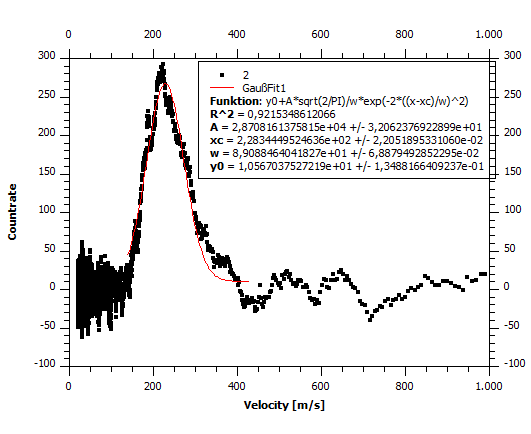
\includegraphics[scale=0.65]{./data/Vel_Spectrum.png}
\caption{Velocity Spectrum with Gaus Fit}
\label{fig:Velocity Spectrum}
\end{figure}
\begin{multicols}{2}



\end{multicols}
\begin{figure}[H]
\centering
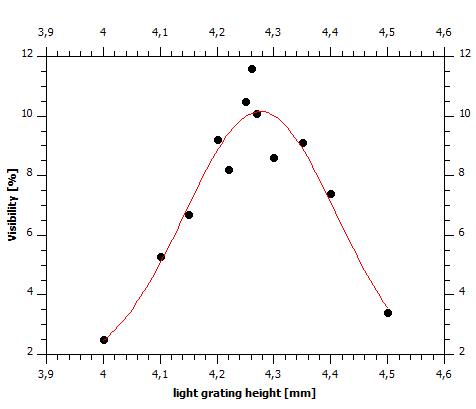
\includegraphics[scale=0.55]{./data/LGH.png}
\caption{Interference as function of the light grating height}
\label{fig:LGH}
\end{figure}
\begin{multicols}{2}

In the end, the visibility was measured as function of the laser power to get as much visibility as possible.
\begin{figure}[H]
\centering
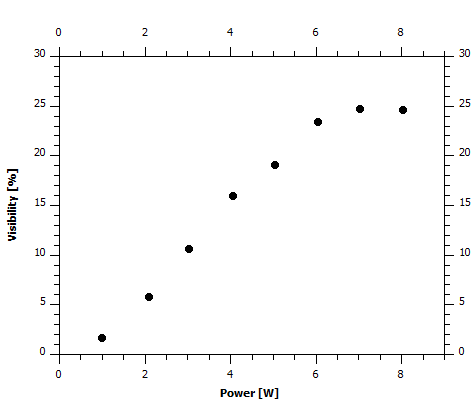
\includegraphics[scale=0.65]{./data/Power.png}
\caption{Interference as functionn of Laserpower}
\label{fig:Laserpower}
\end{figure}

For the calculation of the visibility, a software program written in matlab was used. Alternativly, one can calculate it oneself by fitting a sine curve over the obtained data. For this reason, the data with the maximum visibility was used. The following figure shows the plot. The calculatet visibility is
$24,30\pm0,03$
which is the same as the calculatet visibility by the software program. 

\begin{figure}[H]
\centering
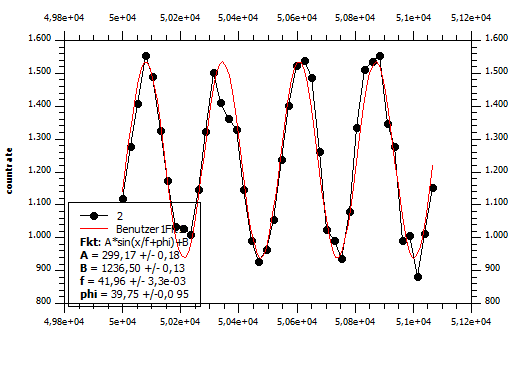
\includegraphics[scale=0.60]{./data/Sinfit.png}
\caption{Calculation of visibility}
\label{fig:Sinfit}
\end{figure}




%\begin{figure}[H]
%	\centering
%	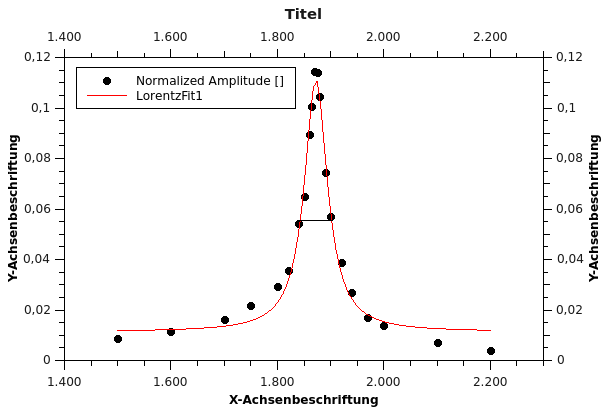
\includegraphics[scale=1]{../figures/Resonanzkurve.png}
%	\caption{Resonanzkurve}
%	\label{fig:resonanzkurve}
%\end{figure}

%%%%%%%%%%%%%%%%%%%%%%%%%%%%%%%%%%%%%%%%%%%%%%%%
%%%%%%%%%%%%%%%%%%%%%%%%%%%%%%%%%%%%%%%%%%%%%%%%
\section{Discussion}
Since it was worked on a real experiment which is currently in use, great causion had to be taken. Therefore, a simulation prior to the actual day in the laboratory had to be done. This simulation was very usefull and a good preparation. It also helped to save time at the day of the experiment. Another positiv effect of using a real experiment is that this helped to decreas the posibility of systematic errors done by false alignment for instance.
The experiment was a success, since we could show interference of large molecules. Thus, we could show the existance of matter waves. The remarkable thing about matter maves is, that classical physics does not provide an explanation for them.  Although, the maximum visibility of approximately 24\% could have been better. 
For this experiment, it is important that the table on which it is standing, is free of vibration. For this reason, it is possibily to levitate the hole table on air. Regretfully one of the pillars broke down the week before our experiment. This could have led to a decrease in the visibility. Moreover, the alignment could have been better to maximise the count rates.

\section{Appendix}

\begin{figure}[H]
\centering
\pgfplotstabletypeset[
columns={Light grating height,Visibility},
col sep=&,
columns/Light grating height/.style={precision=2, zerofill, column name=\makecell{$Light grating height$\\$(\pm 0.1)[mm]$} },
columns/Visibility/.style={column name=\makecell{$Visibility$\\$\pm0.7[\%]$}, precision=0},
every head row/.style={before row=\hline,after row=\hline\hline},
every last row/.style={after row=\hline},
every first column/.style={column type/.add={|}{} },
every last column/.style={column type/.add={}{|} }
]{
Light grating height & Visibility
4 & 2.5
4.5 & 3.4
4.4 & 7.4
4.35& 9.1
4.3 & 8.6
4.25 & 10.5
4.2 & 9.2
4.15 & 6.7
4.1 & 5.3
4.22 & 8.2
4.27 & 10.1
4.26 & 11.6

}
\caption{Light grating height optimization}
\label{tab:LGH}
\end{figure}


\begin{figure}[H]
\centering
\pgfplotstabletypeset[
columns={Laserpower,Visibility},
col sep=&,
columns/Laserpower/.style={precision=2, zerofill, column name=\makecell{$Laserpower$\\$(\pm 0.01)[W]$} },
columns/Visibility/.style={column name=\makecell{$Visibility$\\$\pm0.9[\%]$}, precision=0},
every head row/.style={before row=\hline,after row=\hline\hline},
every last row/.style={after row=\hline},
every first column/.style={column type/.add={|}{} },
every last column/.style={column type/.add={}{|} }
]{
Laserpower & Visibility
0.986	& 1.7
2.079 & 5.8
3.01 & 10.7
4.05 & 16
5.02 & 19.1
6.02 & 23.5
7.02 & 24.8
8.02 & 24.7


}
\caption{Laserpower optimization}
\label{tab:LGH}
\end{figure}




\section{Resources}
\begin{itemize}
	\item Simulation of the Experiment and background information \url{http://interactive.quantumnano.at}
\end{itemize}
Sandra Eibenberger: Diplomarbeit, Kapitza-Dirac-Talbot-Lau Interferometrie mit komplexen Molekülen, Wien 2010
Leitfaden Praktikum Quantenoptik


%\bibliography{protocol.bib}
%\bibliographystyle{plain}

\end{multicols}
\end{document}